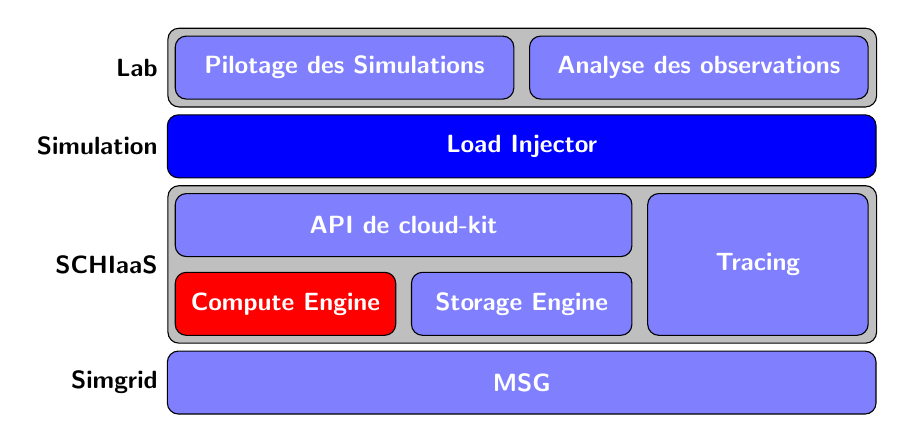
\begin{tikzpicture}[y=1cm,x=3cm,
base/.style={%
outer sep=1mm,
font={\sffamily\bfseries\color{white} \fontsize{9pt}{12}\selectfont},
minimum width=2.8cm,
minimum height=0.8cm,
rounded corners,
fill=blue!50,
anchor = west,
draw,
},
level/.style={%
  font={\sffamily\bfseries\color{black} \fontsize{9pt}{12}\selectfont},
  align=right,
  anchor=east},
mod3/.style={%
base,
outer sep=0,
minimum width=9cm,
},
mod2/.style={%
base,
minimum width=5.8cm,
},
top2/.style={%
base,
minimum height=1.8cm,
},
bg/.style={%
draw,
anchor=west,
rounded corners,
fill=gray!50
},
active/.style={
fill=red,
},
passive/.style={
fill=blue!33,
}
]

%SG
\node[level]at(0,0){Simgrid};
\node[mod3]at(0,0){MSG};

%SCHIaaS
\node[level]at(0,1.5){SCHIaaS};
\node[bg,minimum height=2cm,minimum width=9cm]at(0,1.5){};
\node[base,active]at(0,1){Compute Engine};
\node[base]at(1,1){Storage Engine};
\node[mod2]at(0,2){API de cloud-kit};
\node[top2]at(2,1.5){Tracing};

%Simulator
\node[level]at(0,3){Simulation};
\node[mod3,fill=blue]at(0,3){Load Injector};

%Lab
\node[level]at(0,4){Lab};
\node[bg,minimum height=1cm,minimum width=9cm]at(0,4){};
\node[base,minimum width=4.3cm]at(0,4){Pilotage des Simulations};
\node[base,minimum width=4.3cm]at(1.5,4){Analyse des observations};
\end{tikzpicture}